%!TEX encoding = UTF-8
\documentclass[12pt,a4paper]{jsarticle}
\usepackage[margin=25truemm,truedimen]{geometry}
\usepackage[dvipdfmx]{graphicx}
\usepackage{url}
\usepackage{titling}

\usepackage{layout}

\usepackage[dvipdfmx]{hyperref}
\usepackage{pxjahyper}

\hypersetup{%
colorlinks=true,
linkcolor=black,
citecolor=black,
urlcolor=black
}

\setlength{\droptitle}{-4em}

\title{
  ZIGEN: XR Windowing System\\
  --- VRネイティブ2D\&3D統合デスクトップ環境 --- 
}
\date{\vspace{-5em}}
\begin{document}

\maketitle

\section{背景}

\begin{figure}[htbp]
  \centering
  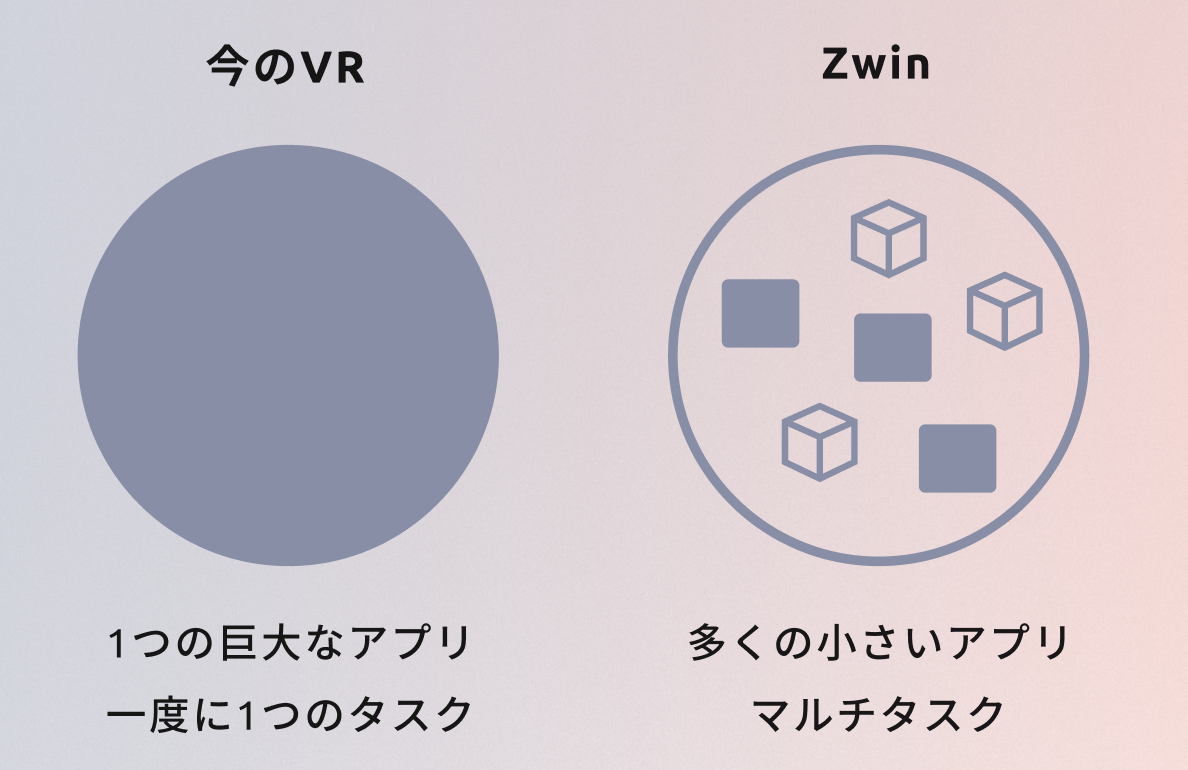
\includegraphics[keepaspectratio, width=0.6\linewidth]{fig/apps.png}
  \caption{既存のVRとZwin(元ZIGEN)とのパラダイムの違い.}
  \label{fig:apps}
\end{figure}

2Dのデスクトップ環境では複数のアプリケーションが同時に使用・連携できるのに対し, 
現状のXRアプリケーションは基本的に1つのメインアプリケーションがユーザの視界の全てを支配する(図 \ref{fig:apps}左).
1つのアプリケーションが1つの世界観を作り出すXRゲームなどにおいてはこれで問題ないが,
特に作業空間や日常生活のサポートとしてのXRでは,全ての機能を1つのアプリケーションが実装するのではなく,
図\ref{fig:apps}右のように個々の機能がそれぞれアプリケーションとして
異なる開発元によって開発され,ユーザが必要な機能のアプリケーションをインストールすることで
自分に最適な作業空間を作れるようにするべきである.

このようにお気に入りのアプリケーションをインストールし,複数のアプリケーションを同時に
利用することで作業空間を作り上げていくことは,2Dのデスクトップ環境では当然のように
行われていることだが,XRの作業空間では達成できていない.
XRにもこのようなマルチアプリケーション・マルチタスクの環境が求められる.

\section{目的}
本プロジェクトの目的はXR空間にWindowing Systemを導入することで
XR空間にマルチアプリケーション・マルチタスクの環境を提供することである.
本プロジェクトは未踏IT人材発掘・育成事業
において,メインのコンセプトについて概念実証をしてきたが,
未踏アドバンストではこれをユーザが日常的に利用できるプロダクトとして実装をすすめ,
認知度の向上と,OSSとしてのプレゼンスを高めることで,Zwin(元ZIGEN)を社会実装していくことである.

\section{製品・サービスの内容}
本プロジェクトではXR Windowing Systemの強みを現状最大限に活かせる環境として,
デスクトップ環境に絞ってプロダクトを開発をした(図\ref{fig:zen}).
特に多くのユーザが利用可能なプロダクトにするため,以下のような開発をした.

\begin{figure}[htbp]
  \centering
  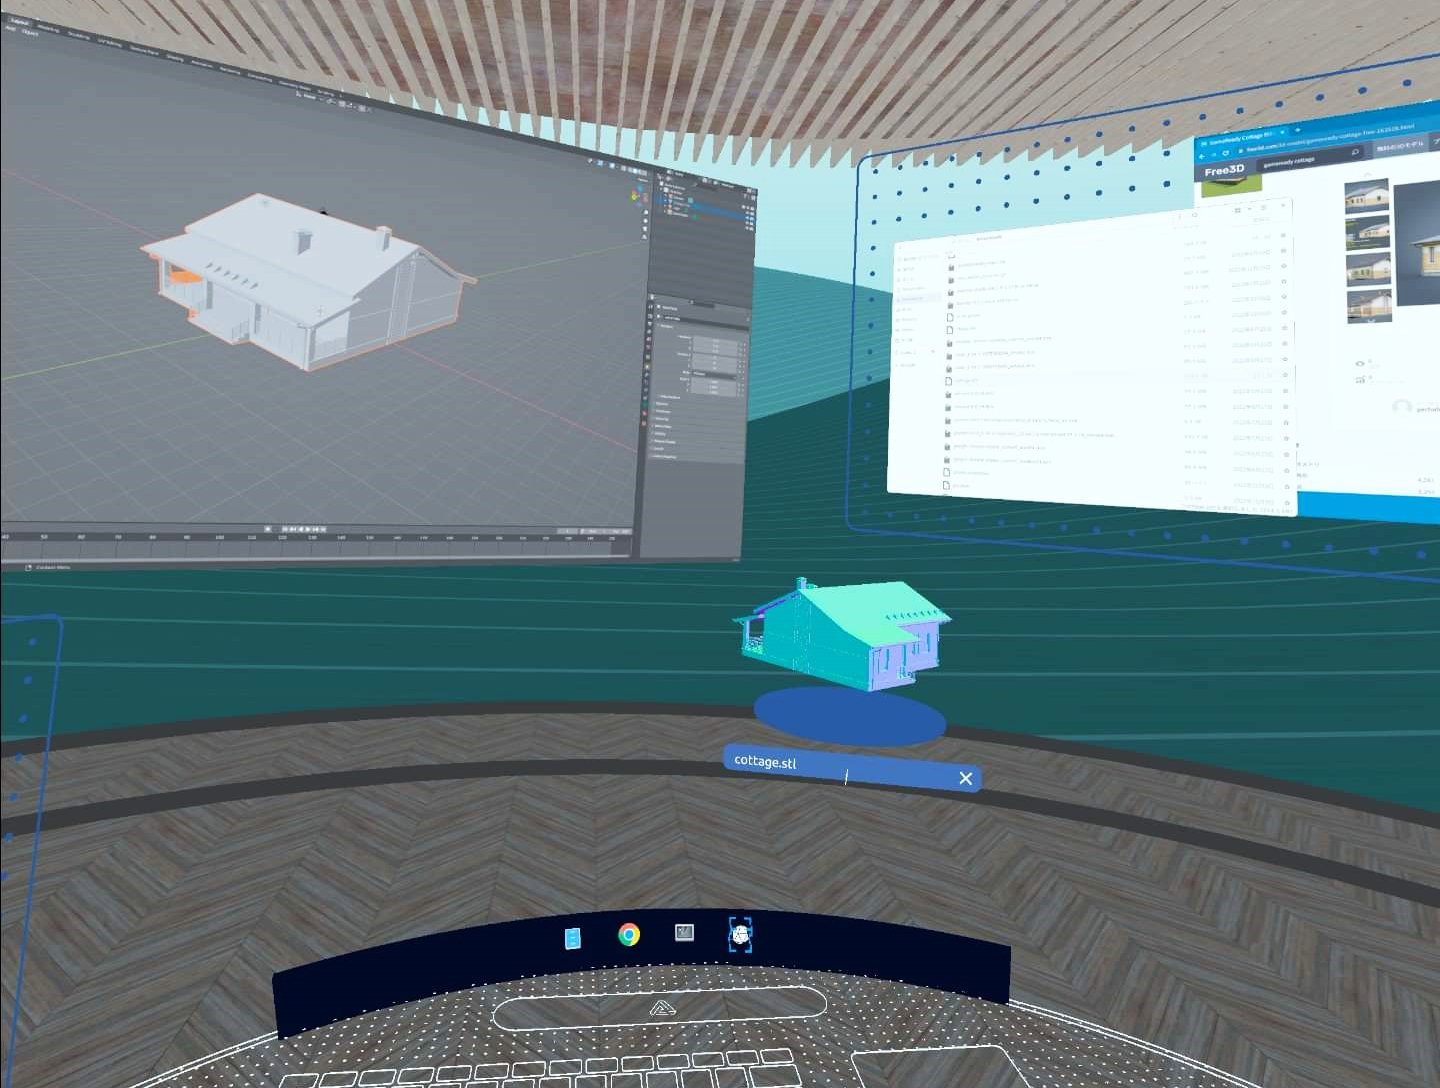
\includegraphics[keepaspectratio, width=0.6\linewidth]{fig/zen.png}
  \caption{本プロジェクトで開発したデスクトップ環境の様子.}
  \label{fig:zen}
\end{figure}

\begin{itemize}
  \item \textbf{Meta Quest 2 への対応} \\
        本プロジェクトの社会実装を進めるためには,利用可能なユーザの母数を増やすことが課題となる.
        2023年1月のSteamの調査
        \footnote{Steamハードウェア&ソフトウェア 調査: January 2023 (accessed on 11 Feb, 2023)}
        によると,VRヘッドセットの利用シェアの44.26\%Meta Quest 2であり,
        プロジェクト実施期間でMeta Quest 2に対応することで,ユーザの母数を増やすことができた.
        Meat Quest2に対応するため,本プロジェクトでは独自にネットワーク越しに
        レンダリングを行う仕組みを実装した.
  \item \textbf{デスクトップ環境の実装} \\
        本プロジェクトではXR Windowing Systemのユースケースをデスクトップ環境に絞った.
        他のユースケースとしては,もっと一般的に歩行中のユーザに様々な情報を提供するような
        システムなどが考えられるが,現状のヘッドセットの重量がまだまだ重い点や,
        既存の2Dアプリケーションというリソースが利用できる点から,デスクトップ環境を選択した.
        プロジェクト実施期間ではデスクトップ環境に必要な,アプリケーションランチャーや
        XR空間で2Dウィンドウをよりうまく利用するためのボードやシート面などの概念を定義し実装した.
  \item \textbf{2Dディスプレイ環境との統合} \\
        未踏アドバンスト事業実施以前のプロトタイプでは,XR空間のみを実装したが,
        XR空間のみではユーザが利用を開始するフローが確立できず,
        またヘッドセットを装着したまま長時間作業を続けることは負担が大きいため,
        プロジェクト実施期間では2Dディスプレイ環境とVR環境との両方のデスクトップ環境を実装し,
        その両者の間を行き来できるようにした.
\end{itemize}

\section{新規性・優位性}

\begin{itemize}
  \item \textbf{2Dと3Dを統合したデスクトップ環境} \\
        VR空間で2Dウィンドウを表示するVRアプリケーションは今までにも多くあるが,
        いずれも既存のOSやWindow Managerを用いて,その上にシステムを構築した.
        この手法ではOSやWindow Managerが提供するAPIに大きな制約うけ,
        ウィンドウの配置などに制約があった.
        Zwinでは2Dデスクトップ環境とXR環境のデスクトップ環境の両方が統合したシステムを
        一から開発することで,そのような制約を受けることなく,またボードという
        2Dデスクトップ環境とXR環境とをスムーズに行き来するための概念を提供できている.
  \item \textbf{3DアプリケーションのためのWindowing Systemのプロトコル} \\
        Zwinでは空間の一部を支配するような小さいアプリケーションが適切にシステムから
        入力を受け取り,自身のコンテンツを没入環境に表示できるWindowing Systemの
        プロトコルを定義している.
        このプロトコルは複数のアプリケーションが同時に没入環境に存在しても競合が最小限になるように
        設計されており,これによって複数の3Dアプリケーションを没入環境で同時に利用できる環境を
        作り上げている.
        このパラダイムを実現することこそが本プロジェクトでもっとも訴求したい新規性となる.
\end{itemize}

\section{事業普及(または活用)の見通し}

事業期間中にベータ版のリリースをし,Twitter上での多くのポジティブなリアクションをいただいた.
実際にインストールした人の感想などを聞くことができた.
ZwinのDiscordサーバの参加者は3倍以上になり,認知度を高めることができた.
海外のYouTubeに他の関連OSSと共に紹介され,関連OSSのDiscordサーバでも
Zwinに言及があるなどOSSとしてのプレゼンスを高めることができた.
また,IssueやPull Requestの形での貢献も受け入れることができ,
ZwinのDiscordサーバでは海外からの参加者を中心に新機能などの議論があり,
OSSとしてのコミュニティ作りも進んでいる.
今後は正式リリースに向けて開発を続け,さらにユーザ,開発者からなるコミュニティを
広げていくつもりである.

\section{期待される波及効果}

2次元のWindowing Systemやスマートフォンの利用者数は40億人程度だと言われている.
今後XRなどの視覚を拡張する情報システムは必ずスマートフォンのように
人々の生活の一部として利用されることになるであろう.
この時,ZwinのWindowing Systemが40億人が利用するシステムの基盤技術なり,
またZwinで検討されたデザインが活用されることを期待する.
ZwinのWindowing Systemの良い点はアプリケーションが空間全体ではなく,
特定の機能だけをうまく実現することが求められるようになることである.
こうして様々な開発者や企業,グループがそれぞれの強みを生かしたアプリケーションを提供し,
参画していくことができるインクルーシブな環境を実現していきたい.

\section{イノベータ名(所属)}
\begin{table}[h]
  \begin{tabular}{ll}
    % textlint-disable
    木内 陽大 & (東京大学大学院情報理工学系研究科)     \\
    江口 大志 & (東京大学大学院情報学環・学際情報学府) \\
    伴 玲吾   & (東京大学大学院情報理工学系研究科)     \\
    渡辺 耀介 & (宇部工業高等専門学校制御情報工学科)   \\
    % textlint-enable
  \end{tabular}
\end{table}

\end{document}
